
\chapter{Automatic Processing User Manual}
\label{chap:usermanauto}

\section{Introduction}

This document is intended to explain the use of the new automatic tracking feature for cracked or damaged records, implemented in PRISM. It explains all options and how to use them when it is possible to automatically track a cracked record.

As a prerequisite, the user must already be familiar with the existing features of PRISM to restore recordings acquired with the 3D Probe.

\section{Overview of the system}

The automatic tracking for cracked records has been created to offer an alternative to a manual system in certain circumstances (see \autoref{sec:autousecase}). To enable this, the procedure is decomposed in several main steps:

\begin{enumerate}
\item Find cracks on the record surface and deduce the main parts separated by cracks, named chunks. There should be no other crack inside a chunk.
\item Proceed with the groove tracking within all chunks.
\item Link the tracked grooves from all chunks and build the final global track, before launching the processing.
\end{enumerate}

For the first step, the configuration impacts the result and may be different regarding the medium type. This particular step is explained in \autoref{sec:setcrackdet}. Also, the linking step often requires the user to check that the final matching results to a proper solution (see \autoref{sec:linkreview}).

\subsection{Typical use cases}
\label{sec:autousecase}

This system works quite well under certain conditions but may fail in the general case. The sought properties for a better result are the followings:

\begin{itemize}
\item The cracks are clearly visible and identifiable (not too thin). This is the case if a significant different of brightness occurs between the regular surface and the crack.
\item The grooves are also identifiable and may be tracked using the depth information. If big scratches occur too often inside a chunk, the tracking may not work properly.
\item For a correct linking, the audio signal should be clearly identifiable, without too many silent part. This point is however not critical as it is possible to manually modify the linking.
\end{itemize}

The cracks detection is based on the properties of the brightness image. The processing then requires that the \emph{.bri} file exists.

\subsection{Configuration panel overview}

A new panel, accessible through the tab \emph{Cracks} has been added next to the detailed view and the interactive panel. It presents all options related to this new tracking method. The main parts of the user interface are visible in \autoref{fig:autoguicontrols} and detailed in \autoref{tab:autoguicontrols}.

\begin{figure}[!ht]
\centering
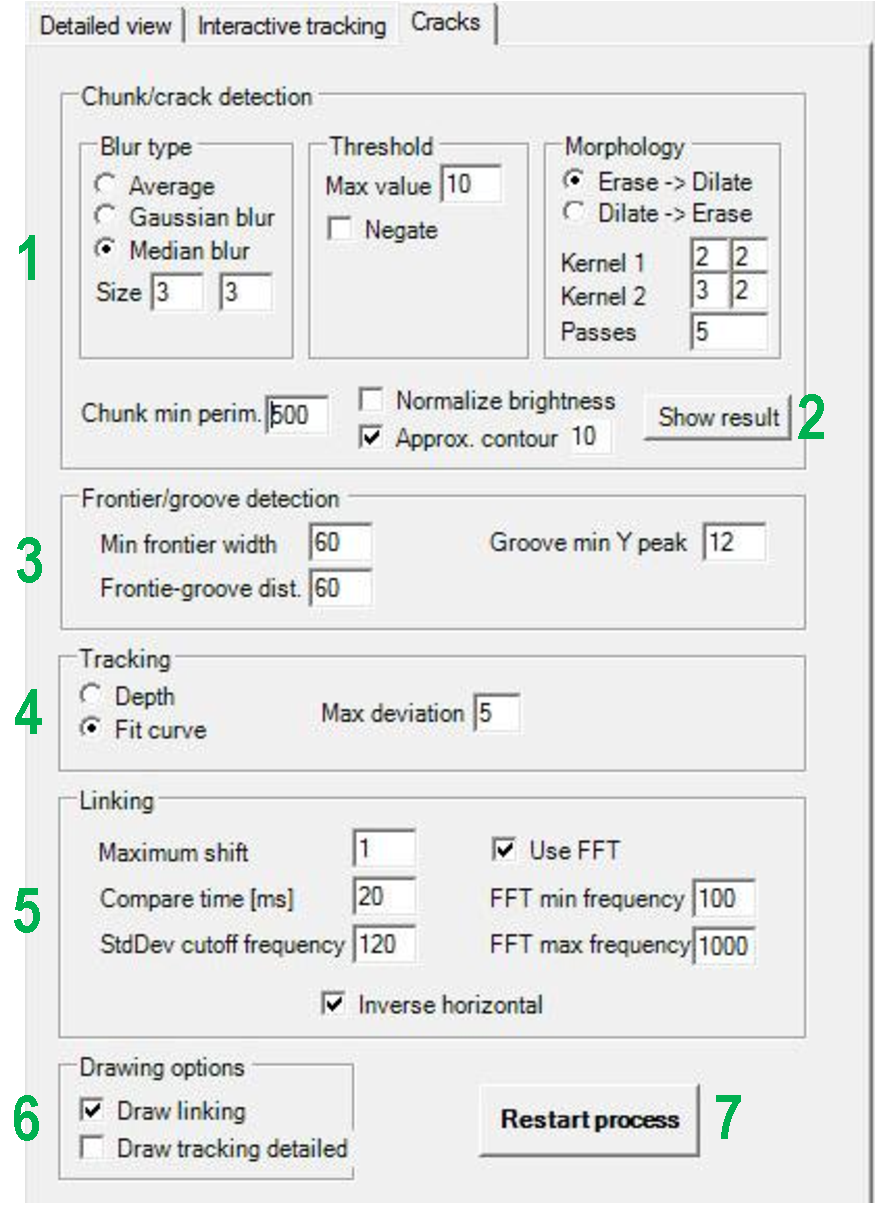
\includegraphics[width=0.45\textwidth]{images/auto-track-controls}
\caption{Visualization of the controls in the \emph{Cracks} panel.}
\label{fig:autoguicontrols}
\end{figure}

\begin{table}[h!]
\begin{center}
\tabulinesep=3pt
\begin{tabu} to 0.8\textwidth {| c | X[m] |} %{>{\bfseries}lX}
    \everyrow{\hline}
    \hline
    \rowfont[c] \bfseries
        No. & Description \\
        1 & Options related to the cracks detection \\
        2 & Enables to show the specific results about cracks detections (if the delimited frontiers are correct) \\
        3 & Options related to groove and frontier detection \\
        4 & Tracking options \\
        5 & Options related to groove linking \\
        6 & Drawing options \\
        7 & Enables to restart the process using the new parameters \\
\end{tabu}
\end{center}
\caption{Explanation of the main parts in the \emph{Cracks} panel.}
\label{tab:autoguicontrols}
\end{table}

\subsubsection{Configuration saving}

All these configurable options are saved in a way similar to the general PRISM options, in an \emph{INI} file. The main difference is that this new file, called \emph{CracksConfig.ini}, is stored locally in the record folder, and not directly the application one.

Indeed, most of the configuration is specific to the current record and it enables to have different saved configurations for each record. It is worth noting that the configuration is loaded at the same time as the record acquisition, and saved back when the application exits. As a consequence, loading a new record overwrites the changes in the configuration. However, the modifications are updated to the file when the processing is restarted (using the button \emph{Restart processing}) or when the program exits.

\section{Starting the cracks detection}
\label{sec:setcrackdet}

First of all, to use this tracking method, one must select the \emph{Cracks auto} tracking option in PRISM which has been added after the existing ones. Then, when loading the record, the program will try to find the cracks, track the record and stop before the final processing. At this point, a view similar to \autoref{fig:cracksdetex} is presented.

\begin{figure}[!ht]
\centering
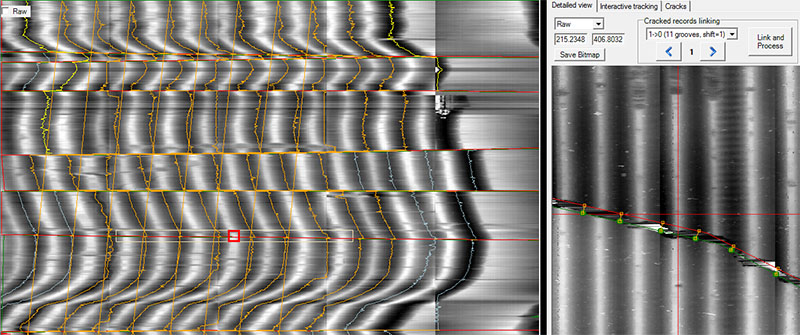
\includegraphics[width=1.0\textwidth]{images/cracks-det-ex}
\caption{Example after loading a record using automatic tracking for cracked records.}
\label{fig:cracksdetex}
\end{figure}

The chunk/crack frontiers are drawn on the binned view as well as the detailed view. On frontiers, small dots represent the detected grooves, as their starting position. The tracking is also visualized on the binned image.

\section{Setting up the cracks detection}

At this point, a complete analysis has already been performed. However, the result may not be correct and satisfactory in the first place. Firstly, we must focus on the cracks detection. All options are located in the cracks panel (\autoref{fig:autoguicontrols}, no. 1).

\begin{description}
\item[Blur type] Should normally not be changed. The median blur is convenient for most cases. If the acquired brightness is very noisy, the size of the blurring kernel may be inscreased (e.g. to $5 \times 5$).
\item[Threshold] This value represents the pixel intensity in the range $[0,255]$ until which it is considered as a crack. This definition is convenient for wax discs or cylinders, where the cracks appear darker than the regular surface. For some recording types, when the cracks appear brighter than the regular surface, the \emph{Negate} option can be used to inverse the result of the thresholding.
\item[Morphology] These options enable to refine the parameters for the morphological operations. For more information, see \autoref{sec:morphop} in the main report. For example, if the cracks are very thin, the dilation kernel may be enlarged, though this will also enlarge the possible noise.
\item[Chunk min perimeter] This value enables to exclude resulting chunks that are too small. The unit is in pixel.
\item[Normalize brightness] Use this option to apply the brightness normalization beforehand (as already implemented in PRISM).
\item[Approximate contours] Enables to approximate the found contours, resulting in a smoother shape. The approximation accuracy may be changed. It represents the maximum distance between the original shape and its approximation.
\end{description}

As this step may require several tests on its own, the final result may be seen in a separate window by clicking on the \emph{Show result} button. The corresponding view is presented in \autoref{fig:autochunkres}.

\begin{figure}[!ht]
\centering
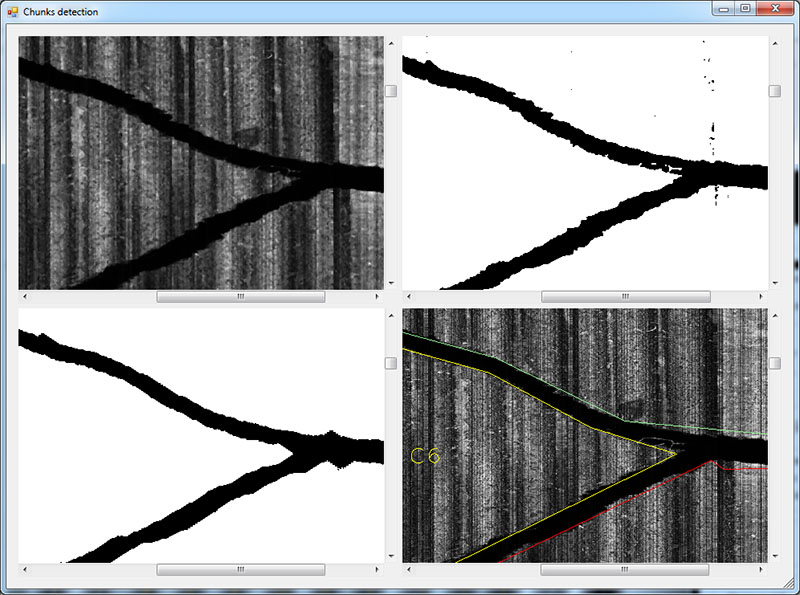
\includegraphics[width=0.8\textwidth]{images/auto-chunk-res}
\caption[Chunk detection visualization.]
{Chunk detection visualization. It shows the result after (from left to right, top to bottom) blurring, thresholding, morphology, and contours detection (drawn over the original brightness image).}
\label{fig:autochunkres}
\end{figure}

This view shows more clearly the result of the different steps applied by the detection algorithm. When the parameters have been adapted, one can apply them by restarting the whole process with the corresponding button and check the result again.

\section{Groove tracking}

Once all chunks are completely detected, the next step is to verify that all grooves are found and correctly tracked. On the binned image, all tracked grooves \emph{inside} a chunk are displayed in light blue. Furthermore, grooves that are already linked to a single track are displayed in yellow or orange (see \autoref{sec:linkreview}).

Thus, if a groove has no line, it has not been found, or the tracking is wrong (may be mingled with another groove).

\subsection{Check groove detection}

To verify if the groove has been found, one can open the detailed view and check whether a green dot appears. An example is viewed in \autoref{fig:automissgroove}.

\begin{figure}[!ht]
\centering
    \begin{subfigure}[t]{0.45\textwidth}
    \centering
    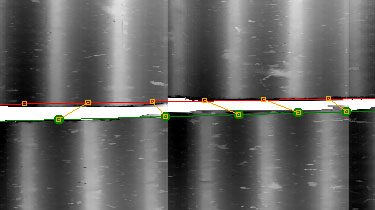
\includegraphics[width=0.9\textwidth]{images/auto-missing-groove}
    \caption{A groove is missing.}
    \label{fig:automiss}
    \end{subfigure}
    \begin{subfigure}[t]{0.45\textwidth}
    \centering
    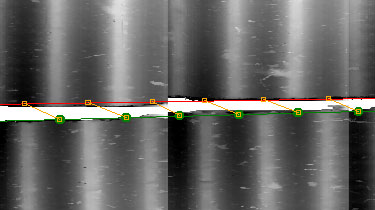
\includegraphics[width=0.9\textwidth]{images/auto-missing-fixed}
    \caption{The problem is fixed.}
    \label{fig:automissfixed}
    \end{subfigure}
    \caption{Example of missing groove as seen on the detailed image.}
    \label{fig:automissgroove}
\end{figure}

In \autoref{fig:automiss}, one groove is not properly detected. The problem is fixed in \autoref{fig:automissfixed}. The useful options for customizing the groove detection are the following (\autoref{fig:autoguicontrols}, no. 3):

\begin{description}
\item[Minimum frontier width] Specifies a minimum width for a frontier to be taken into account. A frontier is either a upper or lower boundary of a crack (for more information, see \autoref{sec:findfrontiers} in the main report). This value may impact grooves detected on small frontiers.
\item[Frontier-groove distance] Specifies the margin size between the detected frontier position and where in the chunk the groove is actually detected. If the surface is particularly noisy around the cracks, this value may be increased.
\item[Groove minimum peak] This value represents the minimum peak height so that it is considered as a groove border. The value corresponds in fact to a percentage from the height difference (which is normalized in the range $[0,100]$ for the detection). If the grooves are heavily embossed, the value may be increased. If they are smaller, a lower value may help to find all grooves but may also find false-positives. For more information about peak detection, see \autoref{sec:groovebot} in the main report.
\end{description}

\subsection{Improve tracking}

Even if the grooves are correctly detected, the tracking sometimes needs to be fixed. Two algorithms are implemented for tracking grooves. The default one, using parabola fitting, usually gives better and smoother results. However, in some cases, the depth fitting may be better suited. The parameter \emph{Max deviation} enables to set the ``dispersion'' of the algorithm, by fixing the maximal deviation from the current position while tracking.

\section{Groove linking}

Finally, the last step is to ensure that the final linking is suitable and results in a well-formed track. An algorithm tries to find the best link using sound analysis. However, tests have shown that it may be wrong. Therefore, after a first automatic step, one must usually manually review the linking.

\subsection{Linking options}

The linking options are used mainly for the automatic linking. The algorithm tries several possibilities and computes a score by comparing the linked sections. The linking with the best score is then selected as the default solution. The parameters are the following (\autoref{fig:autoguicontrols}, no. 5):

\begin{description}
\item[Maximum shift] Represents the maximum shift value tried by the algorithm. For example, if set to 3, the algorithm will compare the current groove with the closest next one, and the three grooves on the left and right (seven tests in total). If it is evident that a record does not suffer a lot from shifting, a smaller value increases the likelihood of a correct linking.
\item[Compare time] Enables to the set the signal length, in \si{\milli\second}, that will be extracted for each sections to be compared to each other. The value in time is independent of the sample rate. Note: for a correct calculation, the RPM option in PRISM must be set correctly.
\item[Use FFT] If checked, the algorithm will compare the spectral domain of the grooves by applying a Fourier transform. Otherwise, the algorithm will compare the standard deviations of the signals, after having applied a high-pass filter.
\item[StdDev cutoff] For standard deviation comparison. Cutoff for the high-pass filter, enabling to get rid of the surface variability not due to the original audio signal.
\item[FFT min/max frequency] For FFT comparison. Minimum and maximum frequency that will be tested on the frequency domain (lower and higher frequencies are usually irrelevant).
\item[Inverse horizontal] This parameter is not related to audio comparison but to how the final tracks are created. Usually, the tracking is performed from left to right. For a tracking starting to the right side, this box must be checked.
\end{description}

Once the options are correctly set, a last pass may be applied by clicking on the button \emph{Restart process}.

\subsection{Linking review and processing}
\label{sec:linkreview}

For the final part, one must go back to the \emph{Detailed view} tab. When the tracking option is created, new controls appear above the record visualization. A list shows parts of chunks that have been linked. When an element of the list is selected, the view is automatically moved to see the corresponding area. The value shows the shift that has been automatically selected.

Then, the shift can be adjusted by pressing on the corresponding buttons. The value is incremented or decremented accordingly, and the result directly changes visually, as seen in \autoref{fig:autodetcontrols}.

\begin{figure}[!ht]
\centering
    \begin{subfigure}[t]{0.45\textwidth}
    \centering
    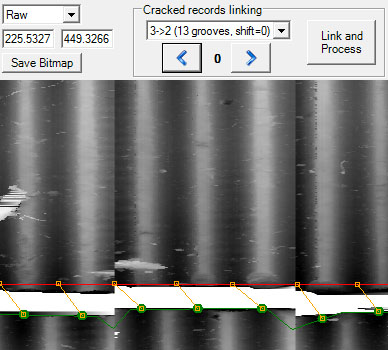
\includegraphics[width=0.9\textwidth]{images/auto-det-controls-1}
    \caption{The shift is set to 0.}
    \label{fig:autodetcontrols1}
    \end{subfigure}
    \begin{subfigure}[t]{0.45\textwidth}
    \centering
    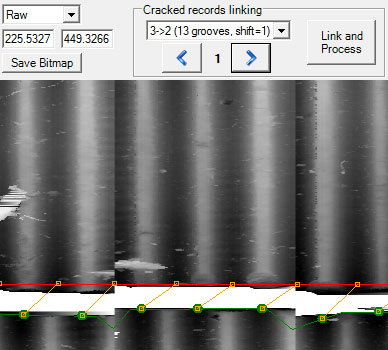
\includegraphics[width=0.9\textwidth]{images/auto-det-controls-2}
    \caption{The shift has been changed to 1.}
    \label{fig:autodetcontrols2}
    \end{subfigure}
    \caption{Controls related to groove linking on the detailed view. The }
    \label{fig:autodetcontrols}
\end{figure}

With this view, it is easy to review the linking to get a final correct result. The path is also displayed on the binned image, enabling to see if the overall result is reasonable. If it is the case, the links from bottom to top are vertical, meaning that the revolution is correct in accordance with the record mapping.

\subsubsection{Final tracks}

The final tracks are drawn in yellow or orange. In fact, this simply enables to distinguish the different tracks. The final result may sometimes lead to multiple tracks. For example, when it is impossible to link a groove in a specific area (record border or no groove to link), the program stops and tries to continue to link another track. An example is shown in \autoref{fig:automulttracks}.

\begin{figure}[!ht]
\centering
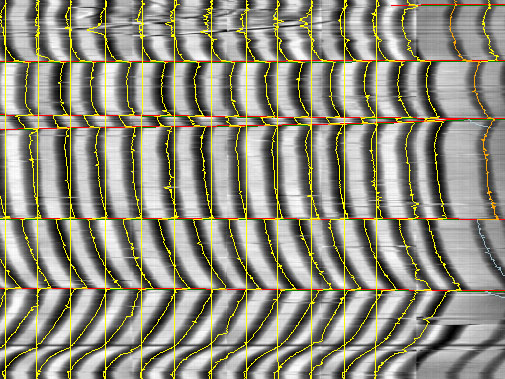
\includegraphics[width=0.8\textwidth]{images/auto-multiple-tracks}
\caption{Multiple tracks as seen on the binned view.}
\label{fig:automulttracks}
\end{figure}

A first small track is drawn in yellow in the upper-left corner of the record. The tracking has then been stopped because the border of the record was reached. The second track (in orange) also stops at the record border. Finally, the rest of the record is properly tracked. One can note that the links are vertical, meaning that the revolutions (from bottom to top) are correctly linked.

\subsubsection{Processing}

Finally, the record may be processed using the existing algorithms by clicking on the button \emph{Link and Process}. As a result, one audio file is created for each track. The name of the files is the usual names with information on the processing, postfixed with \texttt{-track-N}, with $N$ being the track number.

\section{Conclusion}

Using the automatic tracking on a new type of record requires quite a lot of tuning. The results may or may not be adequate regarding the level of damage or the record quality.

This manual gave an exhaustive description of the parameters that may be changed on special situations. However, when applied on a set of similar record that corresponds to the typical use case (see \autoref{sec:autousecase}), it may save a lot of time compared to a fully-manual tracking.

Sometimes, it is also possible that the properties change slightly from a section of a record to another. For best results, it is advisable to process it in several part, by using the ranges appropriately.